\documentclass[10pt]{article}
\usepackage[polish]{babel}
\usepackage[utf8]{inputenc}
\usepackage[T1]{fontenc}
\usepackage{amsmath}
\usepackage{amsfonts}
\usepackage{amssymb}
\usepackage[version=4]{mhchem}
\usepackage{stmaryrd}
\usepackage{graphicx}
\usepackage[export]{adjustbox}
\graphicspath{ {./images/} }

\title{MATEMATYKA }

\author{}
\date{}


\begin{document}
\maketitle
14 MARCA 2018\\
LSCDN

\section*{Instrukcja dla zdającego}
\begin{enumerate}
  \item Sprawdź, czy arkusz zawiera 16 stron (zadania 1-34). Ewentualny brak zgłoś przewodniczącemu zespołu nadzorującego egzamin.
  \item Rozwiązania zadań i odpowiedzi zamieść w miejscu na to przeznaczonym.
  \item Odpowiedzi do zadań zamkniętych (1-25) przenieś na kartę odpowiedzi, zaznaczając je w części karty przeznaczonej dla zdającego. Zamaluj pola do tego przeznaczone. Błędne zaznaczenie otocz kółkiem i zaznacz właściwe.
  \item Pamiętaj, że pominięcie argumentacji lub istotnych obliczeń w rozwiązaniu zadania otwartego (26-34) może spowodować, że za to rozwiązanie nie otrzymasz pełnej liczby punktów.
  \item Pisz czytelnie i używaj tylko długopisu lub pióra z czarnym tuszem lub atramentem.
  \item Nie używaj korektora, a błędne zapisy wyraźnie przekreśl.
  \item Pamiętaj, że zapisy w brudnopisie nie będą oceniane.
  \item Możesz korzystać z zestawu wzorów matematycznych, cyrkla i linijki oraz kalkulatora prostego.
  \item Na tej stronie oraz na karcie odpowiedzi wpisz swój kod (nazwisko i imię - zgodnie z ustaleniami szkolnymi).
  \item Nie wpisuj żadnych znaków w części przeznaczonej dla egzaminatora.
\end{enumerate}

Życzymy powodzenia!\\
Liczba punktów\\
do uzyskania: \(\mathbf{5 0}\)

\section*{Zadanie 1. (1p)}
Rozwiązaniem układu nierówności \(\left\{\begin{array}{c}2 x-4 \leq 6 \\ -x-4<-2\end{array}\right.\) jest zbiór\\
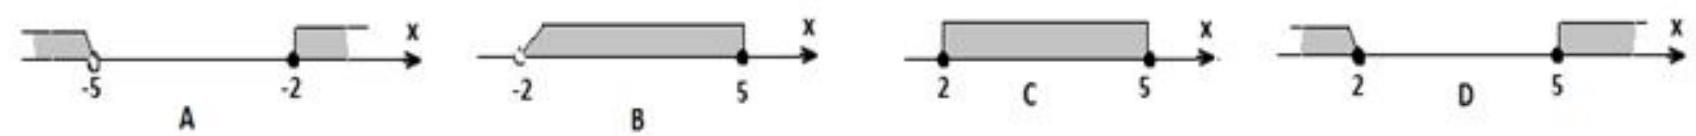
\includegraphics[max width=\textwidth, center]{2024_11_21_19ede52d758866b0d67eg-02}

\section*{Zadanie 2. (1p)}
Wartość wyrażenia \(\frac{\log _{3} 9+2 \log _{3} \sqrt{3}}{2 \log _{2} 4}\) jest równa\\
A. \(\frac{2}{3}\)\\
B. 4\\
C. \(\frac{3}{4}\)\\
D. 9

\section*{Zadanie 3. (1p)}
Cenę towaru obniżano dwa razy. Pierwsza obniżka wynosiła \(10 \%\), a druga 20\%. O ile procent w wyniku obu obniżek spadła cena towaru?\\
A. o 24\%\\
B. o \(28 \%\)\\
C. o \(26 \%\)\\
D. o \(30 \%\)

\section*{Zadanie 4. (1p)}
Jeżeli \(x^{2}-y^{2}=-5\) i \(x-y=5\), to wartość wyrażenia \((x+y)^{2}\) jest równa\\
A. 1\\
B. 16\\
C. 9\\
D. 25

\section*{Zadanie 5. (1p)}
Obrazem rozwiązania układu równań \(\left\{\begin{array}{l}x+y-6=0 \\ x-y+4=0\end{array}\right.\) w prostokątnym układzie współrzędnych na płaszczyźnie jest punkt o współrzędnych\\
A. \((1 ;-5)\)\\
B. \((-1 ; 5)\)\\
C. \((1 ; 5)\)\\
D. \((-1 ;-5)\)

\section*{Zadanie 6. (1p)}
Suma wszystkich pierwiastków równania: \(-(x+5)\left(x^{2}+1\right)(x-7)=0\) jest równa\\
A. 0\\
B. 1\\
C. -2\\
D. 2

\section*{Zadanie 7. (1p)}
Rozwiązaniem równania \(\frac{x+2}{x-2}=3(x \neq 2)\) jest liczba\\
A. 4\\
B. 3\\
C. -2\\
D. -3

\section*{Zadanie 8. (1p)}
Jeśli na rysunku przedstawiony jest wykres funkcji \(\mathrm{f}(\mathrm{x})\), to dziedziną funkcji \(g(x)=f(x-1)\) jest zbiór\\
A. \((-3 ; 4)\)\\
B. \((-3 ; 1)\)\\
C. \(\langle-2 ; 5)\)\\
D. \((-4 ; 3)\)\\
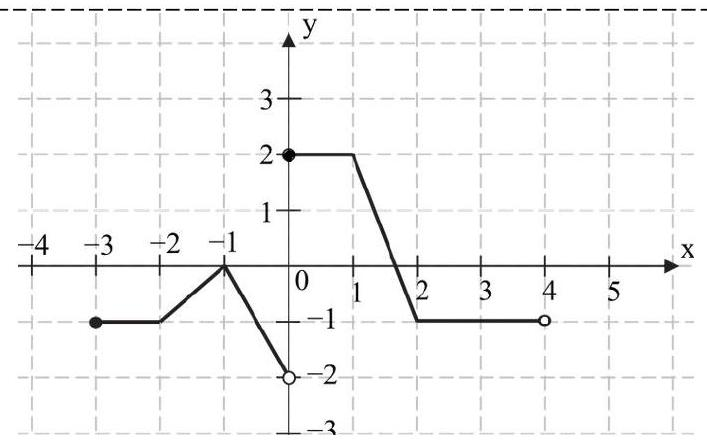
\includegraphics[max width=\textwidth, center]{2024_11_21_19ede52d758866b0d67eg-04(1)}

\section*{Zadanie 9. (1p)}
Funkcja liniowa \(f(x)=a x+x-2\) jest malejąca. Wynika stąd, że\\
A. \(a<-1\)\\
B. \(a<0\)\\
C. \(a>1\)\\
D. \(a>-1\)

Zadanie 10. (1p)\\
Miejsce zerowe funkcji liniowej \(f(x)=(t+1) x-t\) jest równe 2 . Wynika stąd, że\\
A. \(t=-1\)\\
B. \(t=2\)\\
C. \(t=1\)\\
D. \(t=-2\)

Zadanie 11. (1p)\\
Funkcja kwadratowa określona jest wzorem \(f(x)=-x^{2}+2 x+k\). Jeżeli \(f(3)=-6\), to\\
A. \(k=-1\)\\
B. \(k=-3\)\\
C. \(k=-4\)\\
D. \(k=-2\)

\section*{Zadanie 12. (1p)}
Najmniejszą liczbą całkowitą spełniającą nierówność \(\frac{2 x-1}{-2} \leq 3\) jest\\
A. -1\\
B. -3\\
C. -2\\
D. -4

Zadanie 13. (1p)\\
W rosnącym ciągu geometrycznym \(\left(a_{n}\right)\), określonym dla \(n \geq 1\), spełniony jest warunek \(a_{4}=27 a_{1}\). Iloraz \(q\) tego ciągu jest równy\\
A. 2\\
B. 4\\
C. 3\\
D. 5

Zadanie 14. (1p)\\
Jeśli \(\sin \alpha=\frac{1}{4}\), to długość przyprostokątnej \(\boldsymbol{b}\) danego trójkąta (patrz rysunek) jest równa\\
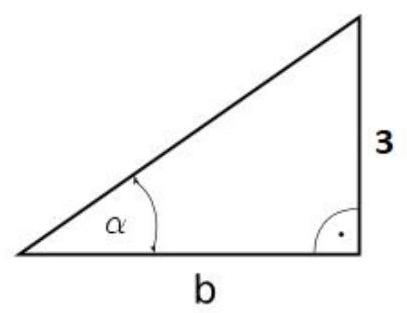
\includegraphics[max width=\textwidth, center]{2024_11_21_19ede52d758866b0d67eg-04}\\
A. \(\sqrt{17}\)\\
B. \(\sqrt{153}\)\\
C. \(\sqrt{140}\)\\
D. \(\sqrt{135}\)

BRUDNOPIS (nie podlega ocenie)

Zadanie 15. (1p)\\
Sinus kąta ostrego \(\alpha\) jest równy \(\frac{1}{3}\). Wówczas \(\operatorname{tg} \alpha\) jest równy\\
A. \(\frac{1}{3}\)\\
B. \(\frac{\sqrt{2}}{4}\)\\
C. \(\frac{1}{4}\)\\
D. \(\frac{\sqrt{2}}{3}\)

Zadanie 16. (1p)\\
W okręgu o środku O dany jest kąt o mierze \(50^{\circ}\) (patrz rysunek). Miara kąta \(\alpha\) zaznaczonego na tym rysunku jest równa\\
A. \(40^{\circ}\)\\
B. \(42^{\circ}\)\\
C. \(45^{\circ}\)\\
D. \(30^{\circ}\)\\
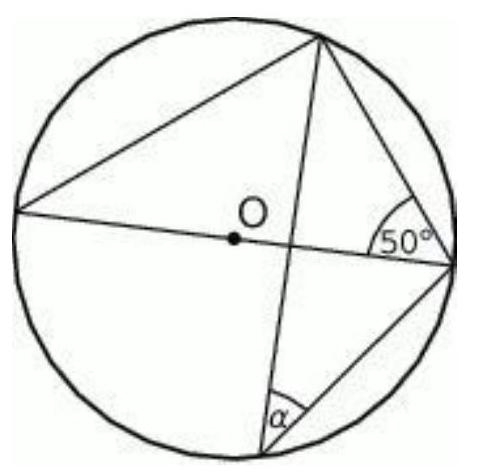
\includegraphics[max width=\textwidth, center]{2024_11_21_19ede52d758866b0d67eg-06}

\section*{Zadanie 17. (1p)}
Przekątna prostokąta ma długość 12 cm i tworzy z jednym z boków kąt o mierze \(30^{\circ}\). Pole powierzchni tego prostokąta jest równe\\
A. \(36 \sqrt{2} \mathrm{~cm}^{2}\)\\
B. \(36 \sqrt{3} \mathrm{~cm}^{2}\)\\
C. \(24 \sqrt{3} \mathrm{~cm}^{2}\)\\
D. \(24 \sqrt{2} \mathrm{~cm}^{2}\)

Zadanie 18. (1p)\\
Proste o równaniach: \(y=a^{2} x-5\) i \(y=\frac{1}{2 a} x+4(a \neq 0)\) są prostopadłe dla \(a\) równego\\
A. 1\\
B. 2\\
C. -2\\
D. -1

Zadanie 19. (1p)\\
Jeśli suma n początkowych wyrazów ciągu arytmetycznego \(\left(a_{n}\right)\) określona jest wzorem \(S_{n}=2 n^{2}+n\), to wartość trzeciego wyrazu tego ciągu jest równa\\
A. 8\\
B. 10\\
C. 12\\
D. 11

Zadanie 20. (1p)\\
Obrazem punktu \(P=(3 ; 4)\) w symetrii środkowej względem punktu \(S\) jest punkt \(P^{\prime}=(-1 ;-2)\) Wynika stąd, że\\
A. \(S=(1 ; 1)\)\\
B. \(S=(-1 ;-1)\)\\
C. \(S=(-1 ; 1)\)\\
D. \(S=(1 ;-1)\)

\section*{Zadanie 21. (1p)}
Powierzchnia boczna walca po rozwinięciu jest kwadratem o polu \(4 \pi^{2}\). Objętość tego walca jest równa\\
A. \(4 \pi^{3}\)\\
B. \(2 \pi^{3}\)\\
C. \(2 \pi^{2}\)\\
D. \(4 \pi^{2}\)

BRUDNOPIS (nie podlega ocenie)

Zadanie 22. (1p)\\
Kula wpisana w sześcian o przekątnej równej 6 cm ma objętość równą\\
A. \(8 \sqrt{3} \pi \mathrm{~cm}^{3}\)\\
B. \(6 \sqrt{3} \pi \mathrm{~cm}^{3}\)\\
C. \(4 \sqrt{3} \pi \mathrm{~cm}^{3}\)\\
D. \(10 \sqrt{3} \pi \mathrm{~cm}^{3}\)

\section*{Zadanie 23. (1p)}
Wszystkich liczb naturalnych dwucyfrowych, w których obie cyfry są nieparzyste jest\\
A. 45\\
B. 25\\
C. 35\\
D. 15

\section*{Zadanie 24. (1p)}
Uczniowie pewnej klasy zostali poproszeni o odpowiedź na pytanie „Ile osób liczy twoja rodzina?" Wyniki przedstawiono w tabeli:\\
Średnia liczba osób w rodzinie dla uczniów tej klasy jest równa 4.\\
Wtedy liczba \(\boldsymbol{x}\) jest równa

\begin{center}
\begin{tabular}{|c|c|}
\hline
\begin{tabular}{c}
Liczba \\
uczniów \\
\end{tabular} & \begin{tabular}{c}
Liczba osób \\
w rodzinie \\
\end{tabular} \\
\hline
6 & 3 \\
\hline
12 & 4 \\
\hline
2 & \(\boldsymbol{x}\) \\
\hline
\end{tabular}
\end{center}

A. 7\\
B. 4\\
C. 5\\
D. 3

Zadanie 25. (1p)\\
Ze zbioru kolejnych liczb naturalnych \(\{1,2,3, \ldots, 25\}\) losujemy jedną liczbę. Prawdopodobieństwo wylosowania liczby, która jest kwadratem liczby całkowitej, jest równe\\
A. \(\frac{5}{25}\)\\
B. \(\frac{6}{25}\)\\
C. \(\frac{7}{25}\)\\
D. \(\frac{4}{25}\)

BRUDNOPIS (nie podlega ocenie)\\

\includegraphics[max width=\textwidth, center]{2024_11_21_19ede52d758866b0d67eg-08}

\section*{ZADANIA OTWARTE}
Rozwiązania zadań o numerach od 26 do 34 należy zapisać \(w\) wyznaczonych miejscach pod treścia zadania (pamiętaj o udzieleniu odpowiedzi)

Zadanie 26. (2p)\\
Rozwiąż nierówność \(-x(x+1)>-12\).

Odpowiedź:

\section*{Zadanie 27. (2p)}
Wykaż, że dla dowolnych liczb rzeczywistych x i y prawdziwa jest nierówność \(x+y \geq \frac{x^{2}+y^{2}+2}{-2}\).

\begin{center}
\begin{tabular}{|c|c|c|c|c|c|c|c|c|c|c|c|c|c|c|c|c|c|c|c|c|c|c|c|c|c|}
\hline
 &  &  &  &  &  &  &  &  &  &  &  &  &  &  &  &  &  &  &  &  &  &  &  &  &  \\
\hline
 &  &  &  &  &  &  &  &  &  &  &  &  &  &  &  &  &  &  &  &  &  &  &  &  &  \\
\hline
 &  &  &  &  &  &  &  &  &  &  &  &  &  &  &  &  &  &  &  &  &  &  &  &  &  \\
\hline
 &  &  &  &  &  &  &  &  &  &  &  &  &  &  &  &  &  &  &  &  &  &  &  &  &  \\
\hline
 &  &  &  &  &  &  &  &  &  &  &  &  &  &  &  &  &  &  &  &  &  &  &  &  &  \\
\hline
 &  &  &  &  &  &  &  &  &  &  &  &  &  &  &  &  &  &  &  &  &  &  &  &  &  \\
\hline
 &  &  &  &  &  &  &  &  &  &  &  &  &  &  &  &  &  &  &  &  &  &  &  &  &  \\
\hline
 &  &  &  &  &  &  &  &  &  &  &  &  &  &  &  &  &  &  &  &  &  &  &  &  &  \\
\hline
 &  &  &  &  &  &  &  &  &  &  &  &  &  &  &  &  &  &  &  &  &  &  &  &  &  \\
\hline
 &  &  &  &  &  &  &  &  &  &  &  &  &  &  &  &  &  &  &  &  &  &  &  &  &  \\
\hline
 &  &  &  &  &  &  &  &  &  &  &  &  &  &  &  &  &  &  &  &  &  &  &  &  &  \\
\hline
 &  &  &  &  &  &  &  &  &  &  &  &  &  &  &  &  &  &  &  &  &  &  &  &  &  \\
\hline
\end{tabular}
\end{center}

\section*{Zadanie 28. (2p)}
Uzasadnij, że jeśli miary kątów wewnętrznych pewnego trójkąta są kolejnymi wyrazami ciągu arytmetycznego, to jeden z tych kątów ma miarę \(60^{\circ}\).\\

\includegraphics[max width=\textwidth, center]{2024_11_21_19ede52d758866b0d67eg-09}

Zadanie 29. (2p)\\
Funkcja kwadratowa o wzorze \(f(x)=-x^{2}+b x+c\) ma dwa miejsca zerowe \(x_{1}=1\) i \(x_{2}=-3\). Wyznacz wartość liczbową współczynników bi c.\\

\includegraphics[max width=\textwidth, center]{2024_11_21_19ede52d758866b0d67eg-10}

Odpowiedź:\\
Zadanie 30. (2p)\\
Oblicz odległość punktu \(K=(24 ; 1)\) od środka odcinka o końcach \(A=(26 ; 18), B=(4 ; 2)\).\\

\includegraphics[max width=\textwidth, center]{2024_11_21_19ede52d758866b0d67eg-10(2)}

Odpowiedź:

\section*{Zadanie 31. (2p)}
W pewnej klasie liczba dziewcząt stanowi \(60 \%\) liczby wszystkich uczniów. Gdyby 6 dziewcząt przeniosło się do innej klasy, w klasie pozostałoby po tyle samo dziewcząt i chłopców. Oblicz ile osób liczy ta klasa oraz ile jest w niej chłopców.\\

\includegraphics[max width=\textwidth, center]{2024_11_21_19ede52d758866b0d67eg-10(1)}

Odpowiedź:

Zadanie 32. (4p)\\
W graniastosłupie czworokątnym prawidłowym przekątna o długości 5 jest nachylona do płaszczyzny podstawy pod kątem \(\alpha\) takim, że \(\sin \alpha=\frac{3}{5}\). Wyznacz objętość tego graniastosłupa.

Odpowiedź:

\section*{Zadanie 33. (4p)}
Doświadczenie losowe polega na dwukrotnym rzucie symetryczną sześcienną kostką do gry. Oblicz prawdopodobieństwo zdarzenia A polegającego na tym, że w pierwszym rzucie otrzymamy nieparzystą liczbę oczek i suma liczb w obu rzutach będzie większa od 6 . Wynik przedstaw w postaci ułamka zwykłego nieskracalnego.\\

\includegraphics[max width=\textwidth, center]{2024_11_21_19ede52d758866b0d67eg-12}

Odpowiedź:

\section*{Zadanie 34. (5p)}
Trzy liczby, których suma jest równa 52, tworzą ciąg geometryczny. Jeśli pierwszą liczbę zmniejszymy o 16 , to otrzymamy ciąg arytmetyczny. Wyznacz te liczby.\\

\includegraphics[max width=\textwidth, center]{2024_11_21_19ede52d758866b0d67eg-13}

Odpowiedź:

BRUDNOPIS (nie podlega ocenie)

\section*{BRUDNOPIS (nie podlega ocenie)}
KARTA ODPOWIEDZI\\
\(\square\) Nazwisko i imię

Wypelnia piszący

\begin{center}
\begin{tabular}{|c|c|c|c|c|}
\hline
\( \underset{\substack{\mathrm{Nr} \\ z \mathrm{za} \text { dania }}}{ } \) & A & B & C & D \\
\hline
1. & ㅁ & ㅁ & ㅁ & ㅁ \\
\hline
2. & ㅁ & ㅁ & ㅁ & ㅁ \\
\hline
3. & ㅁ & ㅁ & ㅁ & ㅁ \\
\hline
4. & ㅁ & ㅁ & ㅁ & ㅁ \\
\hline
5. & ㅁ & ㅁ & ㅁ & ㅁ \\
\hline
6. & ㅁ & ㅁ & ㅁ & ㅁ \\
\hline
7. & ㅁ & ㅁ & ㅁ & ㅁ \\
\hline
8. & ㅁ & ㅁ & ㅁ & ㅁ \\
\hline
9. & ㅁ & ㅁ & ㅁ & ㅁ \\
\hline
10. & ㅁ & ㅁ & ㅁ & ㅁ \\
\hline
11. & ㅁ & ㅁ & ㅁ & ㅁ \\
\hline
12. & ㅁ & ㅁ & ㅁ & ㅁ \\
\hline
13. & ㅁ & ㅁ & ㅁ & ㅁ \\
\hline
14. & ㅁ & ㅁ & ㅁ & ㅁ \\
\hline
15. & ㅁ & ㅁ & ㅁ & ㅁ \\
\hline
16. & ㅁ & ㅁ & ㅁ & ㅁ \\
\hline
17. & ㅁ & ㅁ & ㅁ & ㅁ \\
\hline
18. & ㅁ & ㅁ & ㅁ & ㅁ \\
\hline
19. & ㅁ & ㅁ & ㅁ & ㅁ \\
\hline
20. & ㅁ & ㅁ & ㅁ & ㅁ \\
\hline
21. & ㅁ & ㅁ & ㅁ & ㅁ \\
\hline
22. & ㅁ & ㅁ & ㅁ & ㅁ \\
\hline
23. & ㅁ & ㅁ & ㅁ & ㅁ \\
\hline
24. & ㅁ & ㅁ & ㅁ & ㅁ \\
\hline
25. & ㅁ & ㅁ & ㅁ & ㅁ \\
\hline
\end{tabular}
\end{center}

Razem \(\square\)

\section*{Wypełnia sprawdzający}
\begin{center}
\begin{tabular}{|c|c|c|c|c|}
\hline
\begin{tabular}{c}
Nr \\
zadxuma \\
\end{tabular} & X & 0 & 1 & 2 \\
\hline
26. & \(\square\) & \(\square\) & \(\square\) & \(\square\) \\
\hline
27. & \(\square\) & \(\square\) & \(\square\) & \(\square\) \\
\hline
28. & \(\square\) & \(\square\) & \(\square\) & \(\square\) \\
\hline
29. & \(\square\) & \(\square\) & \(\square\) & \(\square\) \\
\hline
30. & \(\square\) & \(\square\) & \(\square\) & \(\square\) \\
\hline
31. & \(\square\) & \(\square\) & \(\square\) & \(\square\) \\
\hline
\end{tabular}
\end{center}

Razem \(\square\)

\begin{center}
\begin{tabular}{|c|c|c|c|c|c|c|c|}
\hline
\begin{tabular}{c}
Ni \\
zadama \\
\end{tabular} & X & 0 & 1 & 2 & 3 & 4 & 5 \\
\hline
32. & \(\square\) & \(\square\) & \(\square\) & \(\square\) & \(\square\) & \(\square\) &  \\
\hline
33. & \(\square\) & \(\square\) & \(\square\) & \(\square\) & \(\square\) & \(\square\) &  \\
\hline
34. & \(\square\) & \(\square\) & \(\square\) & \(\square\) & \(\square\) & \(\square\) & \(\square\) \\
\hline
\end{tabular}
\end{center}

Razem \(\square\)

\begin{center}
\begin{tabular}{|l|l|}
\hline
Suma punktów & Wynik w\% \\
\hline
 &  \\
 &  \\
\hline
\end{tabular}
\end{center}


\end{document}